\documentclass{article}
\usepackage[utf8]{inputenc}
\usepackage{float}
\usepackage{listings}
\usepackage{enumitem}
\usepackage{todonotes}
\usepackage{pdflscape}
\usepackage[htt]{hyphenat}
\usepackage{minted}
\usepackage{makecell}

\title{MI-FME Cvičení 8}
\author{Tomáš Chvosta}
\date{Březen 2020}

\setcounter{secnumdepth}{-2} % no numbered sections
\usepackage{czech}
\begin{document}

\maketitle

\section{Zadání}
Napište formuli $\Phi_P$ definující přechodovou relaci následujícího programu P:
\begin{figure}[H]
    \centering
    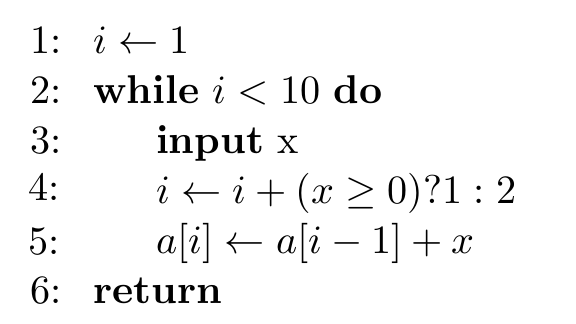
\includegraphics[width=0.4\textwidth]{code.png}
\end{figure}

\section{Řešení}

Přechodová relace $\Phi_P$:
$$[pc=1 \wedge pc' = pc + 1 \wedge i' = 1 \wedge x' = x \wedge a' = a ]$$
$$\lor$$
$$[pc=2 \wedge [i<10 \Rightarrow pc' = pc + 1] \wedge [i \geq 10 \Rightarrow pc' = 6] \wedge i' = i \wedge x' = x \wedge a' = a]$$
$$\lor$$
$$[pc = 3 \wedge pc' = pc + 1 \wedge i' = i \wedge x' = input() \wedge a' = a ]$$
$$\lor$$
$$[pc = 4 \wedge pc' = pc + 1 \wedge [x \geq 0 \Rightarrow i' = i + 1] \ \wedge$$
$$ [x < 0 \Rightarrow i' = i + 2] \wedge x' = x \wedge a' = a ]$$
$$\lor$$
$$[pc = 5 \wedge pc' = 2 \wedge i' = i \wedge x' = x \wedge a' = write(a, i, a[i-1] + x) ]$$
$$\lor$$
$$[pc = 6 \wedge \bot]$$


\end{document}
